\chapter{Controlling Laplacian Eigenfluids}
Many real world applications require us to optimize for some parameters of
a physics-based problem. A toy problem would be to optimize for some initial
angle and velocity of a projectile to hit some target \todo{Refer back to the
learning to throw example}. As a more involved example, \cite{MinDrag} address
finding the best shape of a vehicle to minimize its drag. These kinds of
inverse problems have been around for quite some time in engineering
applications.

Building on all of the previously introduced ideas, we now introduce our
investigation into the use of eigenfluids in fluid control problems, making use
of their explicit closed form description of a velocity field (\todo{link to
equation}). Our main proposition is to achieve reduced-order modeling-like
speed-increase: in lieu of representing the fluid as a grid, we reconstruct the
velocity field only at discrete points in space, while simulating the dynamics
of the fluid in a reduced dimensional space.\todo{Link to eq.}

\section{Our Experiments}
In the following, we showcase different optimization scenarios, where we try out
different aspects of controlling eigenfluids via \acf{DP} gradients. (See
section~\ref{dp-loss}.)

The first couple of examples are "traditional" optimization scenarios. By
"traditional", we mean finding individual solutions to problems via gradient
descent optimization. Moving further, we look for generalized solutions to a set
of problems by training \acfp{NN}.

We implemented all of our experiments in $\Phi_{Flow}$
by \cite{holl2019pdecontrol}.

\subsection{Finding Initial Velocities}
To verify feasibility before moving on to more involved setups, our most
straightforward optimziation scenario is to find an initial basis coefficient
vector $\vb{w}_0 \in \mathbb{R}^N$ for an eigenfluid simulation using $N=16$
basis fields, such that when simulated for $t$ time steps, the reconstructed
$\text{Reconstruct}(\vb{w}_t) = \vb{u}_t$ velocity field will match some
precalculated $\vb{u}^*$ target velocity field.

We initialized the coefficients to random numbers, and ran the eigenfluid
simulation for $t$ timesteps.

Around $100$ steps of \ac{GD} optimization with $\lambda=10^{-3}$ got the loss
under $1.0$, $200$ steps to under $4*10^{-4}$, and each further step was still
continuously decreasing the error. 

\begin{figure}
  \label{fig:finding-initial-velocities}
  \centering
  \begin{subfigure}{\textwidth}
    \centering
    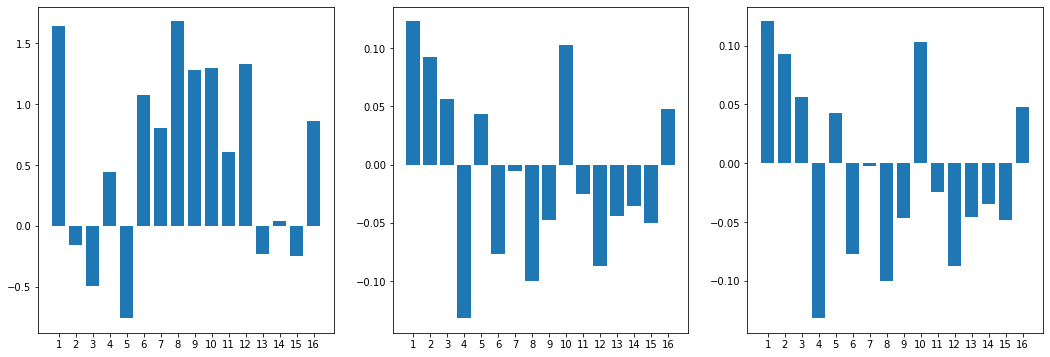
\includegraphics[width=0.9\textwidth]{figures/finding-initial-velocities/t_16_coefficients.png}
    \caption{$\vb{w}_{init}$, $\vb{w}_{optim}$, and
    $\vb{w}^*$, optimizing for velocity field after $16$ timesteps}
  \end{subfigure}\par\medskip
  \begin{subfigure}{\textwidth}
    \centering
    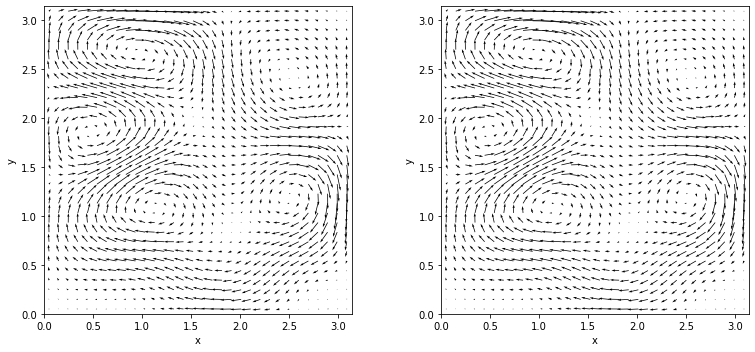
\includegraphics[width=0.8\textwidth]{figures/finding-initial-velocities/t_16_velocities.png}
    \caption{Target $\vb{u}^*$, and $\vb{u}^{16}$, reconstructed from
      $\mathcal{P}^{16}(\vb{w}_{optim})$\\}
  \end{subfigure}\par\medskip
  \begin{subfigure}{\textwidth}
    \centering
    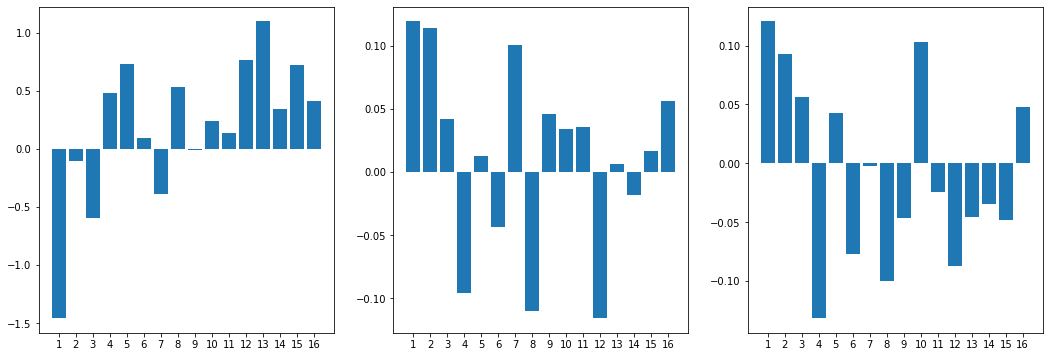
\includegraphics[width=0.9\textwidth]{figures/finding-initial-velocities/t_100_coefficients.png}
    \caption{Initial basis coefficients $\vb{w}_{init}$, $\vb{w}_{optim}$, and
    $\vb{w}^*$, optimizing for velocity field after $100$ timesteps\\}
  \end{subfigure}\par\medskip
  \begin{subfigure}{\textwidth}
    \centering
    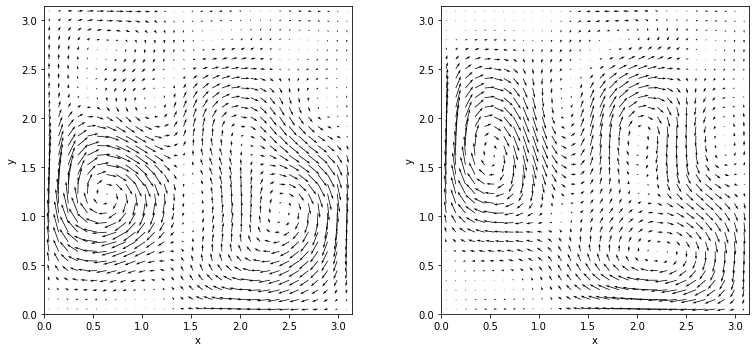
\includegraphics[width=0.8\textwidth]{figures/finding-initial-velocities/t_100_velocities.png}
    \caption{Target $\vb{u}^*$, and $\vb{u}^{100}$, reconstructed from
      $\mathcal{P}^{100}(\vb{w}_{optim})$}
  \end{subfigure}
  \caption{Results of optimizing for an initial $\vb{w}_0$ basis coefficient
  vector that matches a target velocity field $\vb{u}^*$ when reconstructed
  after simulating for $t$ time steps.}
\end{figure}

Naturally, this very basic method has its limits. Trying to find the same
coefficients based on a simulated velocity field after $t=100$ timesteps proved
to be a substantially harder problem, as even a relatively small error can
accumulate into major deviations over these longer timesteps, resulting in much
less stable gradients.  With using the same learning rate, the optimization
diverged almost instantly. With some manual tuning of the learning rate
$\lambda$, we were able to get the loss below $0.14$. (Starting from an initial
loss of $320$ from the random initialization.) 

We visualize the results of these two scenarios in
Figure~\ref{fig:finding-initial-velocities}. It is interesting to observe that
even though the optimization had absolutely no knowledge of $\vb{w}^*$, only
a comparison with a precomputed $\vb{u^*}$ velocity field at timestep $100$, the
optimized $\vb{w}_{optim}$ vector already starts to look similar to $\vb{w}^*$.
Keep in mind that this is not guaranteed at all, as highlighted with the
\todo{link to learning to throw example}. 

Although there are a number of ways to tweak this setup, from these results, it
is already evident from these scenarios that the flow of gradients working,
and is ready to be tested in more advanced scenarios.

\subsubsection*{Matching a Grid-based Fluid Simulation}

\subsection{Controlling Shape Transitions}
\label{section:controlling-shape-transitions}
\todo{Formulate problem, loss function, etc here}

\subsubsection*{Sampling}
\todo{Write about sampling strategies of points, how shapes are defined, etc.}

\subsubsection{Initial Velocity}
\todo{Move some parts of this under main
Section~\ref{section:controlling-shape-transitions}}

In the following, we will showcase an optimization scenario, where we try to
find an initial base coefficient vector $\vb{w}^{0}$ for an eigenfluid
simulation with $N=16$ basis fields, such that when simulated for $t$ time
steps, the reconstructed velocity field will advect a set of initial points
$\vb{p}^0 = [p^0_0\dots p^i_0]$ to line up with target positions 
$\vb{p}^{t} = [p^t_0\dots p^t_i]$. We can write this optimization problem as 

$$\arg\min_{\vb{w}} \text{Loss}(\vb{w}, \vb{p}^0, \vb{p}^t)
= \arg\min_{\vb{w}} \left| \mathcal{P}^{t}(\vb{p}^0, \vb{w})
- \vb{p}^t\right|_2^2 = \arg\min_{\vb{w}}
\sum_{i}\left|\mathcal{P}^{t}(p^0_i, \vb{w}) - p^t_i\right|_2^2, $$

where $\mathcal{P}^t(\vb{w}, \vb{p}) = \underbrace{\mathcal{P} \circ
\mathcal{P} \dots \circ \mathcal{P}(\vb{w}, \vb{p})}_{t \text{ times}}$
denotes the physical simulation of base coefficients $\vb{w}$ and 
points $\vb{p}$ in the velocity field reconstructed from $\vb{w}$. We
use a simple mean-square error (also known as $L_2$ norm) for measuring the error.

The main difficulty of this non-linear optimization problem lies in that we have
no control over the natural flow of the fluid besides supplying an initial
$\vb{w}^0$ vector.

Making use of the differentiability of our physical simulator $\mathcal{P}$, and
the multivariable chain rule for deriving the gradient of the above
$\mathcal{P}^t$ function composition, we can derive its gradient with respect to
the initial coefficients:
$$\frac{\partial \mathcal{P}^t(\vb{w},\vb{p})}{\partial \vb{w}}.$$

Finally, we can simply iterate a gradient descent optimizer with learning
rate $\mu$ to find a (good enough) solution for our above minimization problem:

$$\vb{w}_{\text{better}} = \vb{w} - \mu
\frac{
    \partial\text{Loss}(\vb{w}, \vb{p}_0, \vb{p}^t)
}{
    \partial \vb{w}
}$$

\subsubsection{Control Force Estimation}
\todo{Write only about problem statement + optimization part for optimizing
for $f \in \mathbb{R}^{t \times N}$ force vector.}
\todo{Move this section a bit up in the hierarchy? Where?}
\todo{Write about generalizing the CFE to arbitrary shapes via training a NN.}

\subsubsection{Neural Network Training}
